\section{The A3-E Model}\label{sec:proposal}

\begin{figure}[tbp]
	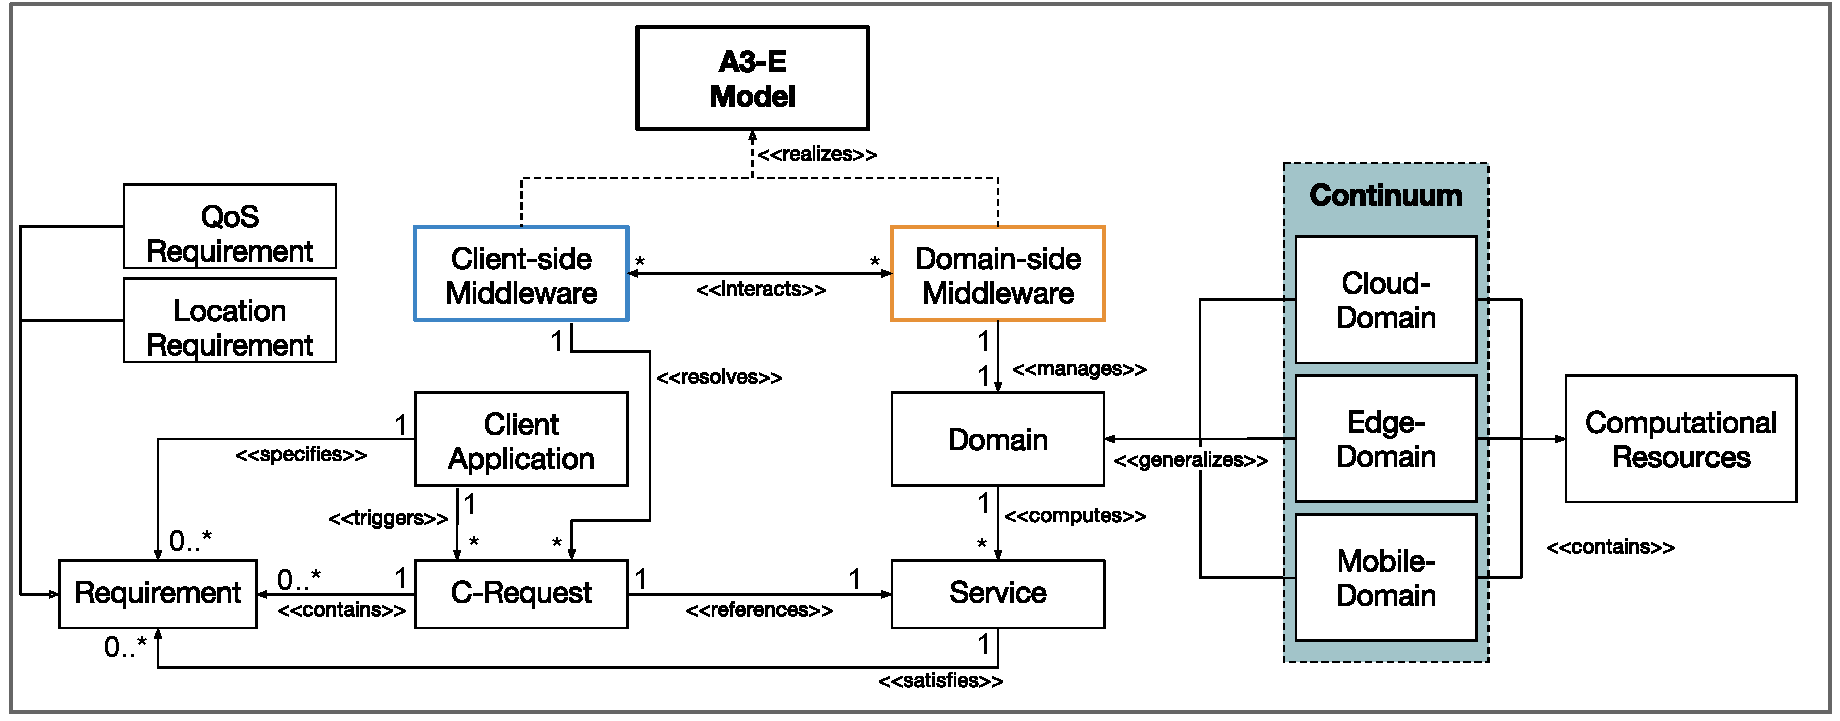
\includegraphics[width=0.95\textwidth]{figs/A3-E-model.pdf}
	\caption{The A3-E Model.}
	\label{fig:A3-E-model}
\end{figure}

As depicted in Fig.~\ref{fig:A3-E-model}, the A3-E model consists of the different concepts and mechanisms required for the realization of the cloud-edge-mobile continuum. Its name inherits from the four phases process -- namely, \textit{(\textbf{A}wareness), (\textbf{A})cquisition, (\textbf{A})llocation, and (\textbf{E})ngagement} -- employed both by clients and the different types of computational resources composing the continuum. 

The A3-E model also encompasses the concepts of client applications, services and service requirements, as well as those of a client-side and a domain-side middleware. In specific, the client-side middleware is responsible for proxying requests from client applications and forwarding them to the domain that best satisfies the service requirements in a given moment and situation. In turn, the domain-side middleware is responsible for the self-management of services life-cycle in a given domain. Last but not least, the constituents of the continuum (i.e., cloud datacenters, edge servers, and mobile devices) are represented in the model by the following domain refinements: cloud-domain, edge-domain, and mobile-domain.

\subsection{A3-E Process}\label{sec:A3-E-process}

\begin{figure}[tbp]
	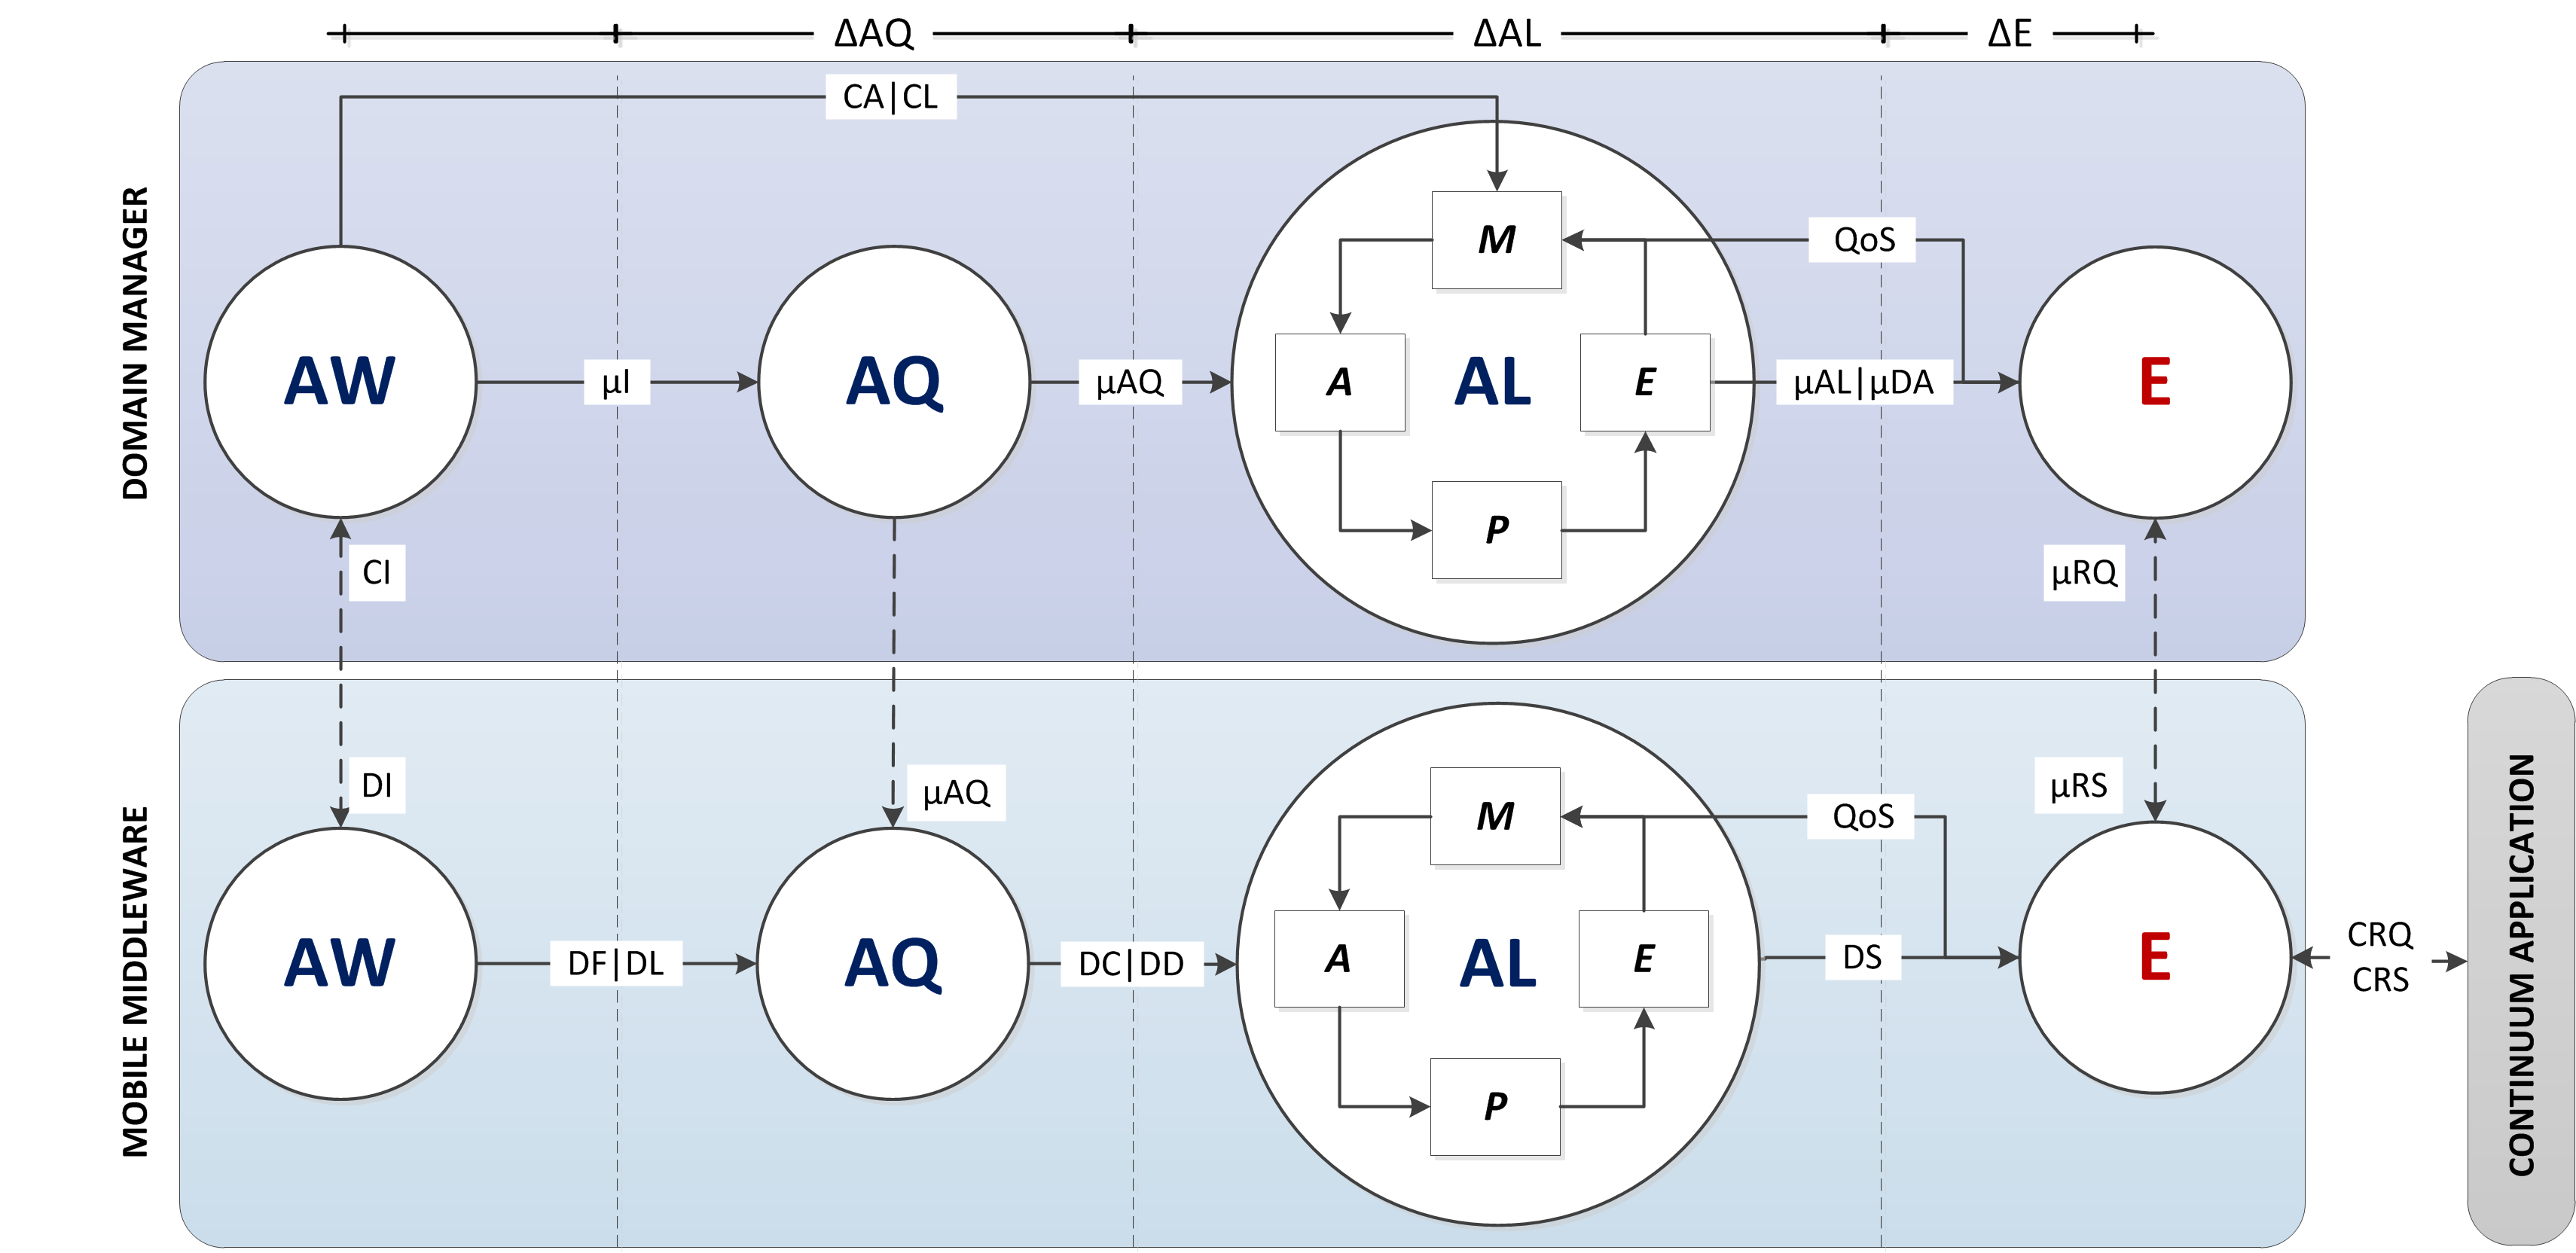
\includegraphics[width=0.9\textwidth]{figs/A3-E.png}
	\caption{The A3-E Process. Phases are delimited by vertical lines and the main activity of each phase by the label within each phase; labels within parenthesis represent the states of a domain to a client (and vice-versa)}
	\label{fig:A3-E-process}
\end{figure}

%What: the process within A3-E
The A3-E process is composed of four phases. Each of these phases is refined by activities -- performed by the client-side and domain-side middlewaress -- that take care of specific concerns in the interaction among client applications and the compute continuum.

A3-E is flexible with respect to its process phases and addresses all the constituents of the compute continuum. In specific, the diagram in Fig.~\ref{fig:A3-E-model} represents the scenario in which a domain first contacts an application hosted by a mobile client. This particular instance of the A3-E model is used to illustrate the use of all four phases in the model. Later on, other possible instances of the A3-E model are correlated with scenarios of the compute continuum.

%Next, the four A3-E phases are further described and mapped to the requirements elicited in  Section~\ref{sec:requirements}. Later on, other possible instances of the A3-E model are correlated with scenarios of the compute continuum.

\subsubsection*{Awareness Phase}\label{sec:A3-E-awareness}

%Why do we need awareness?
%CA: awareness is not needed because the edge domain should always be coupled to the network infrastructure; network components shoudl aways route traffic to existing edge servers; additionally, the edge domain should be able to acquire and allocate services upon detection of the first requests.  
%A: A3-E model is agnostic w.r.t. the use of network technologies to route traffic to the edge servers; a given domain my count on network components to traffic route to its servers instead of negociating directly with clients aware of its existance; nonetheless, the lack of awareness limits the acquisition and deployment of services to reactive, as the domain would only identify a given service upon the first request has been made. Clients, in the other hand, would not be able to choose from alternative domains. 

In A3-E, the Awareness phase has the following purposes: 1) to enable a domain to pro-actively initialize other phases (namely acquisition and allocation) based on its awareness about  applications hosted by clients in the domain coverage area (Requirement Rx); and 2) to enable clients to choose from alternative domains based on their awareness about these domains (Requirements Ry).

%From the domain side, the lack of awareness of clients in the domain coverage area prevents triggering the acquisition and subsequently allocation phases based on this event. From the client side, the lack of awareness from surrounding domains prevents them to make the decision of which domains to use. In the later case, clients must rely on external components to reach servers (e.g., traffic managers and DNS servers).

\subsubsection*{Acquisition Phase}\label{sec:A3-E-acquisition}

The Acquisition phase has the following purposes: 1) to enable a domain to pro-actively install artifacts used by services that must become available in that domain (Requirement R2); and 2) to enable clients to pro-actively identify their requirements (services) and allow the domain to pro-actively install them (Requirement Rx).

%From the domain side, the lack of acquisition implies that service assets must be previously made available. Nonetheless, the preliminary acquisition of a large number of assets is limited by the domain storage capability. 

%Conversely, the automated and opportunistic acquisition of service assets improves storage efficiency with the cost of a setup time $\Delta_{AQ}$. For instance, domains that become aware of clients' requirements may pro-actively start the acquisition phase and become ready for allocation before the first service request arrives.

%otherwise, domains must rely on the detection of a first service request or some other triggering condition to start the acquisition phase and, after setup time $\Delta_A$, become ready for allocation. 

\subsubsection*{Allocation Phase}\label{sec:A3-E-allocation}

The allocation phase has the following purposes: 1) to enable the automated process of making a service ready for execution through the allocation of computational resources (Requirement R1); and to enable clients to choose among different alternative domains that may be available (Requirement Ry).
 
%Cloud providers already implement automated scaling mechanisms, e.g, with the allocation of virtual machines and container instances on demand. More recently, the FaaS model introduced zero-allocation mechanism, in which stateless functions may remain deallocated until they are invoked (cold start). Once the demand increases, the FaaS platform may respond with additional instances of the required functions.

%From the domain side, A3-E adheres to the dynamic allocation of computational resources for services execution. Applications that can not afford the delay (hereafter named $\Delta_{AL}$) of a cold start must rely on services that are always kept available with minimum allocation. Instead, whenever cold start is acceptable, the zero-allocation provides a more efficient usage of computational resources. Needless to say, $\Delta_{AL}$ is only perceived by the first request after a cold start, while subsequent calls are processed normally hereafter.

%From the client-side, once the awareness phase has been active and identified the current alternative domains, the client may consider QoS values from each domain to make the decision of which one to engage. Conversely, the lack of awareness implies that client engagement with a specific domain must be solved by means of a well-known name. In the later case, the network backbone is responsible for routing client requests to specific domains.

\subsubsection*{Engagement Phase}\label{sec:A3-E-engagement}

Finally, the \textit{engagement} phase models the actual interaction between a client and a service. At this stage, the requested service must be already acquired and allocated for execution. 

%What: how different policies may be employed by domains and clients throughout A3-E-Process
\subsection{Phase Transitions and Policies}

\begin{figure}[tbp]
	\raggedright
	\subfloat[Different states of a given edge domain with respect to a given client application; the transitions between states triggered by domain events are guarded by policies that may vary according to the type of edge infrastructure and the service level agreement (SLA)\label{fig:A3-E-domain}] {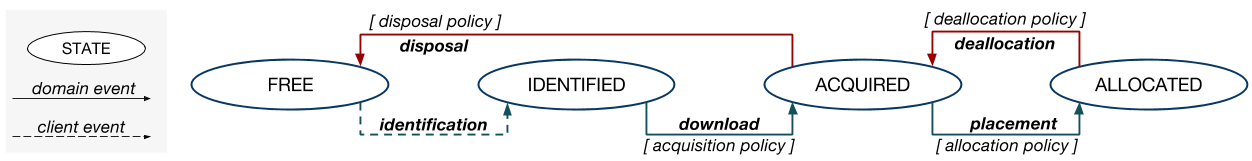
\includegraphics[width=0.95\textwidth]{figs/A3-E-domain.png}}\hfill
	
	\subfloat[Different states of a given client with respect to a given edge domain; the transitions between states triggered by client events are guarded by policies that may vary according to the client requirements\label{fig:A3-E-client}] {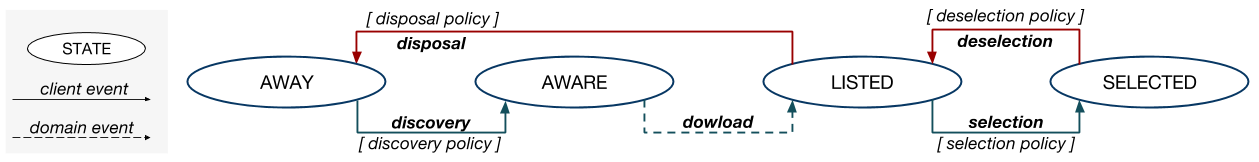
\includegraphics[width=0.95\textwidth]{figs/A3-E-client.png}}\hfill
	\caption{States and transitions among A3-E phases} \label{fig:A3-E-states}
\end{figure}

%What: the flexibility of A3-E model in terms of policies that regulate the transition among phases

The A3-E model is also flexible with respect to the transitions among subsequent phases. In particular, distinct policies may define different transition behaviors. Figures~\ref{fig:A3-E-domain} and~\ref{fig:A3-E-client} depict, respectively, the possible transitions among states of a domain with respect to a client application and vice-versa. Each state is mapped to the corresponding phase in Fig.~\ref{fig:A3-E-model}. 

Above all, policies affect the following conflicting properties: a) the \textit{efficiency} of domain resource usage (domain side); and b) the application tolerance for service setup \textit{delay} (client side). Considering the first request arrival ($FRA$) from a client application as the reference event, the more \textit{reactive} the policies are to that event, the less time domain resources are likely to remain idle before it happens (more efficiency). In contrast, the chances of underutilization and idleness are higher with \textit{proactive} policies (less efficiency). Eq.~\ref{eq:setup_cost} models the total delay of service setup:

\begin{equation}\label{eq:setup_cost}
C_{SETUP} = C_{OFFLINE} + C_{RUNTIME}
\end{equation}

\noindent
in which the first term ($C_{OFFLINE}$) represents the resources required for downloading and installing the services (e.g., network and storage), whilst the later ($C_{RUNTIME}$) represents the resources needed for executing the services (e.g., memory and CPU). 

From the delay point of view, the relation is the opposite: the more \textit{reactive} the policies are with respect to the first request arrival event, the higher the delay the first request to each service is served with. In the other direction, the more \textit{pro-actively} services are made ready for execution, the lower the delay the first request to each of these services is served with. Eq.~\ref{eq:setup_delay} models the total delay of service setup:

%\Delta_{NET} + 
\begin{equation}\label{eq:setup_delay}
L_{SETUP} = \Delta_{AW} + \Delta_{AQ} + \Delta_{AL}
\end{equation}

\noindent
in which the first term ($\Delta_{AW}$) represents the time it takes for clients and domains to become aware of each other. The second term ($\Delta_{AQ}$) represents the time for acquiring all assets of a specific service, whilst the last term ($\Delta_{AL}$) represents the time for allocating resources for the service execution. 

For instance, existing cloud-based FaaS platforms (e.g., Amazon Lambda, Google Cloud Functions, and Apache OpenWhisk) employ on demand allocation of stateless functions, i.e., functions are reactively allocated upon arrival of the first request. Depending on the policy configuration, the platform waits for an idleness interval before deallocating the function~\cite{}. In these cases, the improved efficiency of the platform in allocating computational resources has the drawback of a setup delay (cold start). Next, the domain-side policies in Fig.~\ref{fig:A3-E-domain} are categorized.

\subsubsection*{Domain Policies} The domain-side policies in Fig.~\ref{fig:A3-E-domain} can be refined into three types: \textit{proactive (P)}, \textit{sequential (S)}, and \textit{reactive (R)}. The employment of each type during acquisition and allocation is described as follows:

\begin{itemize}
	
\item Acquisition

\begin{itemize}

\item \textbf{Proactive}: acquisition phase starts upon external event preceding the $FR_A$ event (e.g., the prediction of service usage in the near-future). Benefits: first response delay ($FR_D$) does not include $\Delta_{AQ}$. Drawback: acquired artifacts remain idle until usage. Example: stateless functions required by body device applications during a marathon event are fetched the night before the event by mobile-edge domains located along the course. 

\item \textbf{Sequential}: the beginning of acquisition phase is dictated by the completion of the awareness phase. Benefits: service artifacts are only acquired upon detection of a potential client in the domain coverage area, minimizing the likelihood of idleness. Drawbacks: $FR_D$ may include a fraction of $\Delta_{AQ}$ if $FRA$ precedes the end of acquisition. Example: stateless functions to be consumed by a mobile multiplayer game application are acquired by an indoor-edge domain inside a passenger train upon detection of two or more clients in the train.

\item \textbf{Reactive}: acquisition phase starts upon detection of a $FRA$. Benefits: acquisition of service artifacts follows an actual demand, eliminating artifacts storage idleness. Drawbacks: $FR_D$ includes $\Delta_{AQ}$, which may be disruptive for some applications. Example: stateless functions to be consumed by a TODO 
\medskip
\medskip
\bigskip
\bigskip

%the notion of a reactive allocation can be extended also to the acquisition of service artifacts. Instead of having functions pre-downloaded and installed, this process could happen in reaction to the first arrival of a request. 

\end{itemize}
\end{itemize}

\begin{itemize}

\item Allocation

%The \textit{allocation policies} in Fig.~\ref{fig:A3-E-domain} can be:

\begin{itemize}

\item \textbf{Proactive}: allocation phase starts upon external event preceding the arrival of the first request (e.g., the prediction of service usage in the near-future). Benefits: $FR_D$ does not include $\Delta_{AL}$. Drawback: allocated resources remain idle until $FR_A$. Example: stateless functions to be consumed by connected vehicles are pre-allocated by mobile-edge domains in specific day times.

\item \textbf{Sequential}: allocation phase starts as soon as acquisition phase finishes. Benefits: depends on the acquisition policy. Drawbacks: depends on the acquisition policy. Example: stateless functions required by a marathon application running on body devices are allocated following their acquisition by the mobile-edge domains along the course.

\item \textbf{Reactive}: allocation phase starts as soon as $FR_A$ is detected. Benefits: eliminates idleness by conditioning allocation to an actual service demand. Drawback: $FR_D$ includes $\Delta_{AL}$ (cold start). Example: stateless functions required by a mobile multiplayer game are allocated by a local-edge domain inside a train following the detection of a $FR_A$ event.

\end{itemize}
\end{itemize}


%In the opposite direction, both \textit{deallocation} and \textit{disposal policies} can either be:
%
%\begin{itemize}
%
%\item Proactive: deallocation/disposal is triggered upon external event (e.g., triggered by a prediction of ); ; 
%
%\item Reactive: allocation phase starts as soon as the first request for a service arrives (cold start).
%
%\end{itemize}


%The client must either have opted for that specific domain during allocation phase or, in case of awareness/allocation has not been employed by the client, it must rely on external components to route its request to a given domain in a transparent way.

%the start of the allocation phase may be triggered by the end of the acquisition phase, or it may be combined with additional conditions required for the allocation phase to start.
%
%For instance, the awareness of a client application, which may happen pro-actively through the awareness phase, may be the additional condition for the allocation phase to start. In this case, allocation may finish before the first request to arrive, eliminating the delay of a cold start.
%
%For instance, a client would engage with a cloud service by firing a request to a well-known Internet name. At some point of the network infrastructure (e.g., at the cellular base station), a component diverges the request to the edge servers in that domain.
%
%In contrast, a local-edge domains may advertise its existence to clients in connection range. Each client, upon awareness of multiple domains (in this case, the edge and the cloud), decides which domain to use. If the client QoS requirement is network latency, the decision should favor the local-edge. 


%The acquisition-allocation transition, in its turn, is modelled by two alternative policies: 
%
%\begin{itemize}
%
%\item proactive allocation: phase starts as soon as acquisition phase finishes; or
%
%\item reactive allocation: phase starts as soon as acquisition phase finishes and the client notifies its intention for using that domain.
%
%\end{itemize}
%
%Finally, reverse transitions are single and dependent on the specific policies for deallocating and disposing of application assets. 
%In accordance with Requirement R6, the aforementioned policies are useful for different classes of applications, as well as different types of edge computing infrastructure and different usage contexts.
%
%


%\subsection{A3-E Instances}\label{sec:A3-E-instances}

\begin{center}
\begin{table}[htbp]
\small
\caption{Domain-side instances of the A3-E model corresponding to parts of the cloud-edge-mobile continuum (CTN) with corresponding awareness mechanisms (\textbf{W}ell-\textbf{K}nown-\textbf{N}ame or \textbf{A}dvertisement\&\textbf{D}iscovery) and policies (\textbf{P}roactive, \textbf{S}equential, \textbf{R}eactive) that may be employed for triggering the acquisition and allocation in each instance. }\label{tab:A3-E-instances}
\begin{tabular}{ c c c c c c }
\toprule

CTN & E.M. & \textbf{A}WARENESS & \textbf{A}CQUISITION	& \textbf{A}LLOCATION 	& \textbf{E}NGAGEMENT  	\\

\midrule

\multirow{2}{*}{ Cloud }
& IaaS	& W.K.N.	& OFFLINE		& HOT-START	& BY REQUEST\\
& FaaS		& W.K.N.	& OFFLINE		& COLD-START	& BY REQUEST\\\midrule					
\multirow{2}{*}{ Edge }
& FaaS		& W.K.N.	& [P, R]		& [P, S, R] 	& BY REQUEST\\
& FaaS		& A\&D	& [P, S, R]		& [P, S, R]		& BY REQUEST\\\midrule	
\multirow{1}{*}{ Mobile }
& FaaS	& LOCAL  & OFFLINE	& HOT-START 	& BY REQUEST\\

\bottomrule
\end{tabular}
\end{table}
\end{center}
\normalsize

Table~\ref{tab:A3-E-instances} correlates the possible domain-side instances of the A3-E model with different parts of the cloud-edge-mobile continuum along with the approach used for awareness and the policies~\footnote{The policy adopted by a phase affects which policies may be adopted by its subsequent phase (e.g., a reactive acquisition implies a reactive allocation, as service assets must first be acquired before been deployed, whilst a proactive acquisition may be combined with a reactive allocation).} depicted in Fig.~\ref{fig:A3-E-domain} that may be adopted in each case. 


\subsection{A3-E Instances}

By taking into account the conflicting properties of \textit{efficiency} and \textit{delay}, we envision the following mapping between A3-E instances and scenarios composing the cloud-edge-mobile continuum:

--- \textbf{Cloud-IaaS}. Services hosted in the cloud are, in most of the cases, reachable by means of a well-known Internet name (therefore, no dynamic awareness is employed). Assets used by these services are preliminarily deployed to cloud servers (thus, no dynamic acquisition is employed). Virtual machines and containers are pre-allocated (hot start), and cloud's elasticity mechanisms take care of the (de)allocation of resources according to a service level agreement (SLA). Finally, cloud services are invoked by clients (engagement phase). Target services: delay-tolerant and stateful computation; persistence.

--- \textbf{Cloud-FaaS}. The FaaS model distinguishes from the cloud instance described above by enforcing the use of stateless functions that can be quickly allocated for execution without minimum pre-allocation (cold start). Targeted services: delay-tolerant and stateless computation.

--- \textbf{Edge-Opportunistic}. Services hosted in the edge, in contrast, may need to opportunistically advertise their existence (awareness phase), acquire application assets (acquisition phase), make them ready for invocation (allocation phase), before finally been able to expose the required computation as services to be consumed. In this case, the policies employed for acquisition and allocation may vary between proactive, sequential, or reactive. Targeted services: non-critical applications with desirable requirements for low-latency.

--- \textbf{Edge-Critical}. The later modality of edge computing may co-exist with others in which: 1) services are transparently accessed through well-known Internet names; 2) service assets are pre-acquired (offline acquisition); and 3) services are pre-allocated in order to increase the readiness required by certain types of applications (hot start). Targeted services: critical applications with strict requirements for low-latency.

--- \textbf{Mobile}. This last instance represents the local computation performed by mobile devices. It provides a zero network latency with high availability; in contrast, the resource constraints of mobile devices may result in lower processing performance and undesirable battery drain, therefore justifying the use of other instances (mobile computation offloading), unless none is available. Targeted services: latency-sensitive and lightweight computation.

Finally, clients may also adopt different policies for the discovery and selection. In particular, the policies in Fig.~\ref{fig:A3-E-client} can be:

\begin{itemize}

\item \textbf{Discovery policies (Awareness)}:

\begin{itemize}
	
	\item TODO: ...; or
	
	\item TODO: ...
	
\end{itemize}

\item \textbf{Selection policies (Allocation)}:

\begin{itemize}
	
	\item TODO: ... or
	
	\item TODO: ...
	
\end{itemize}
\end{itemize}

%TBW: Example with one of the applications mentioned in the motivation (AR/CV).

\subsection{Reference Architecture}

Figure~\ref{fig:reference-architecture} shows the proposed architecture for the compute continuum. Particular focus is put on the interaction between devices and Edge domain servers, since it is the main contribution of this paper. 
The main physical elements are mobile devices and domain servers. Mobile devices can be of any type (e.g., tablets, smartphones), running several low-latency applications that needs offloading part of their computation to more powerful servers. For this, the devices send information to be processed to the domain server through standardized network protocols~\cite{Sill17standards}.  A Base Transceiver Station\footnote{Different generations of wireless mobile networks use distinct names (e.g., eNodeB in 4G).} (BTS) bridges mobile devices and domain servers as a part of the cellular infrastructure and  Edge architecture, according to its current specifications~\cite{hu2015mobile}. In this scenario, mobile devices and Edge domain servers are at no more than a few hops from each other. These servers host a serverless infrastructure, where stateless functions are deployed and executed according to the phases defined by the A3-E model. 
The following sections provide details about the A3-E middleware (Section~\ref{subsec:A3-E}) and the serverless infrastructure that materializes Edge domain servers (Section~\ref{subsec:ServerlessArchCont}).

\begin{figure}[tbp]
	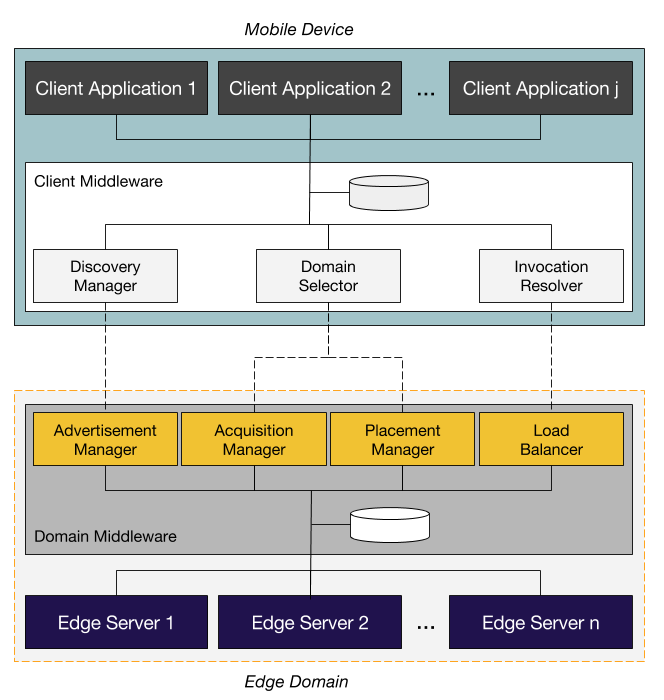
\includegraphics[width=.6\textwidth]{figs/reference-architecture.png}
	\caption{A3-E architecture in Mobile Devices and Edge Domains TODO: UPDATE THIS DIAGRAM}
	\label{fig:reference-architecture}
	\end{figure}